\documentclass[conference, 12pt]{IEEEtran}
% \IEEEoverridecommandlockouts
% The preceding line is only needed to identify funding in the first footnote. If that is unneeded, please comment it out.
\usepackage{cite}
\usepackage{amsmath,amssymb,amsfonts}
\usepackage{algorithmic}
\usepackage{graphicx}
\graphicspath{{assets/}}
\usepackage{textcomp}
\usepackage{xcolor}
\def\BibTeX{{\rm B\kern-.05em{\sc i\kern-.025em b}\kern-.08em
    T\kern-.1667em\lower.7ex\hbox{E}\kern-.125emX}}
\begin{document}


\title{USO DE LA SIMULACION PARA EL ESTUDIO DEL COMPORTAMIENTO DEL COVID}

\author{\IEEEauthorblockN{Rafael Morales Venegas}
\IEEEauthorblockA{\textit{Universidad Tecnológica Metropolitana}\\
Santiago, Chile}
% \and
% \IEEEauthorblockN{Santiago C. Zapata}
% \IEEEauthorblockA{\textit{Profesor de Optimización de Sistemas} \\
% \textit{Universidad Tecnológica Metropolitana}\\
% Santiago, Chile}
}

\maketitle

\setlength\parskip{1.5\baselineskip}

\begin{abstract}
    La pandemia del COVID-19 ha sido un problema que ha enfrentado la humanidad desde ya inicios de 2020, un poco más de dos años. Para evitar muertes humanas y la desestabilidad económica de múltiples regiones, científicos de todo el mundo han trabajo en el desarrollo de modelos matemáticos de todo tipo, junto con variadas simulaciones de los mismos, para el estudio del comportamiento de esta pandemia, al igual que la asistencia en la toma de decisiones para cumplir estos objetivos.

    Este documento presenta una introducción al uso de modelos matemáticos y simulaciones en el estudio de la epidemia del COVID-19 en el mundo, junto con un análisis breve de sus resultados.
\end{abstract}

\begin{IEEEkeywords}
    % No estoy del todo seguro de esto. @TODO
COVID, Modelos, Optimización de Sistemas, Toma de Decisiones
\end{IEEEkeywords}

% Este archivo gobierna la primera sección correspondiente únicamente
% a la introducción.

\section{Introduction}
This document is a model and instructions for \LaTeX.
Please observe the conference page limits. 

\section{Marco teórico}
Se ofrecen, entonces, las siguientes definiciones como sustento o marco teórico para este documento:

%%%%%%%%%%%%%%%%%%%%%%%%%%%%%%%%%%%%%%%%%%%%%%%%%%%%%%%%%%%%%%%%%%%%%%%%%%%%%%%%%%%%%

\subsection{Modelo}
Es una representación abstracta de un sistema, utilizada comúnmente para el estudio del mismo. Para efectos de este documento, nos referiremos específicamente a Modelos de tipo Matemáticos, o séa, representaciones matemáticas de sistemas.

%%%%%%%%%%%%%%%%%%%%%%%%%%%%%%%%%%%%%%%%%%%%%%%%%%%%%%%%%%%%%%%%%%%%%%%%%%%%%%%%%%%%%

\subsection{Sistema}
Conjunto de elementos que interactúan entre sí.

Conjunto de reglas o principios sobre una materia racionalmente enlazados entre sí.

Conjunto de 'cosas' que, relacionadas entre sí de forma ordenada, contribuyen a determinado objeto.

%%%%%%%%%%%%%%%%%%%%%%%%%%%%%%%%%%%%%%%%%%%%%%%%%%%%%%%%%%%%%%%%%%%%%%%%%%%%%%%%%%%%%

\subsection{Sistema abierto}
Es un sistema que interactúa con su entorno.

%%%%%%%%%%%%%%%%%%%%%%%%%%%%%%%%%%%%%%%%%%%%%%%%%%%%%%%%%%%%%%%%%%%%%%%%%%%%%%%%%%%%%

\subsection{Sistema cerrado}
Es un sistema que no interactúa con su entorno.

%%%%%%%%%%%%%%%%%%%%%%%%%%%%%%%%%%%%%%%%%%%%%%%%%%%%%%%%%%%%%%%%%%%%%%%%%%%%%%%%%%%%%

\subsection{Subsistema}
Los sistemas pueden ser compuestos por otros sistemas menores o más pequeños, que en interación de unos con otros producen el sistema mayor.

%%%%%%%%%%%%%%%%%%%%%%%%%%%%%%%%%%%%%%%%%%%%%%%%%%%%%%%%%%%%%%%%%%%%%%%%%%%%%%%%%%%%%

\subsection{Modelo determinístico}
Es un modelo cuyas relaciones siempre producen el mismo comportamiento cuando reciben la misma 'entrada'. Esto quiere decir que el sistema no tiene elementos aleatoreos que lo componen. En este tipo de modelos, las variables internas y de salida quedan determinadas cuando se definan las variables de entrada, parámetros y variables de estado, por lo que las relaciones funcionales entre las mismas están siempre bien definidas.

%%%%%%%%%%%%%%%%%%%%%%%%%%%%%%%%%%%%%%%%%%%%%%%%%%%%%%%%%%%%%%%%%%%%%%%%%%%%%%%%%%%%%

\subsection{Modelo estocástico}
Es un modelo donde una o más relaciones está basada en elementos aleatóreos, lo que implica comportamientos múltiples bajo una misma entrada para el modelo. La idea de estos modelos es representar un sistema con un comportamiento más caótico, como una máquina tragamodenas: en este sistema, la misma entrada (colocar una moneda) genera resultados completamente distintos siempre, por lo que el modelo debe ser capaz de representar esto mediante el uso de aleatoreidad y resultados inciertos.

Es importante recalcar que, si un modelo determinístico es utilizado con entradas estocásticas, su comportamiento será equivalente al de un modelo estocástico.

%%%%%%%%%%%%%%%%%%%%%%%%%%%%%%%%%%%%%%%%%%%%%%%%%%%%%%%%%%%%%%%%%%%%%%%%%%%%%%%%%%%%%

\subsection{Simulación}
Consiste en estudiar el comportamiento de un sistema a través de el uso de un modelo que lo represente. Ambos deben comportarse de manera similar, de tal manera de que el comportamiento del modelo sea fiel a lo que se espera que sea el comportamiento del sistema dado los mismas entradas, y por lo mismo, la simulación depende totalmente de la calidad del modelo para ser exitosa.

%%%%%%%%%%%%%%%%%%%%%%%%%%%%%%%%%%%%%%%%%%%%%%%%%%%%%%%%%%%%%%%%%%%%%%%%%%%%%%%%%%%%%

\subsection{Simulación continua}
Es aquella simulación en el que el estado del modelo cambia permanentemente en el tiempo. Ocurre cuando las relaciones funcionales entre las variables del sistema solo permiten que el estado se transforme en el tiempo de manera continua.

%%%%%%%%%%%%%%%%%%%%%%%%%%%%%%%%%%%%%%%%%%%%%%%%%%%%%%%%%%%%%%%%%%%%%%%%%%%%%%%%%%%%%

\subsection{Simulación discreta}
Es aquella simulación en el que el cambio de estado se produce cada cierto intervalo de tiempo. Los modelos de este tipo se caracterizan porque las variables cambian únicamente en un instante determinado o secuencia de instantes, y permanecen constantes el resto del tiempo.

%%%%%%%%%%%%%%%%%%%%%%%%%%%%%%%%%%%%%%%%%%%%%%%%%%%%%%%%%%%%%%%%%%%%%%%%%%%%%%%%%%%%%

\subsection{Flujo}
"Corriente", o "ir de un lado a otro". En general, el término de flujo se utiliza cuando se hace referencia al movimiento de algo.

%%%%%%%%%%%%%%%%%%%%%%%%%%%%%%%%%%%%%%%%%%%%%%%%%%%%%%%%%%%%%%%%%%%%%%%%%%%%%%%%%%%%%

\subsection{Software}
Conjunto de programas, instrucciones y reglas informáticas para ejecutar tareas en una computadora.

%%%%%%%%%%%%%%%%%%%%%%%%%%%%%%%%%%%%%%%%%%%%%%%%%%%%%%%%%%%%%%%%%%%%%%%%%%%%%%%%%%%%%

\subsection{Hardware}
Conjunto de elementos físicos o materiales que constituyen una máquina. Para el contexto, se refiere particularmente a los que componene a una computadora o sistema informático.

%%%%%%%%%%%%%%%%%%%%%%%%%%%%%%%%%%%%%%%%%%%%%%%%%%%%%%%%%%%%%%%%%%%%%%%%%%%%%%%%%%%%%


\section{Sobre el COVID-19}
Antes de empezar a desarrollar sobre los mecanismos de modelación y simulación de la Pandemia del COVID-19, es necesario hablar más detalladamente del virus.

\subsection*{Mecanismos de Transmisión}
El principal método de transmisión para este virus consiste en el transmisión por 'gotitas'. Una persona infectada al momento de respirar o toser impulsa una cantidad de gotitas y pequeñas particulas que contienen el virus. Estas gotitas pueden y son respiradas por otras personas, o caer en ojos, nariz o boca, o incluso contaminar las superficies que estas toquen, lo que puede generar una infección en esta nueva persona previamente sana. \cite{cdc_2021}

La CDC lista principalmente 3 formas en que este virus se esparce:

\begin{itemize}
    \item "Al inhalar estando cerca de una persona infectada que exhala pequeñas gotitas y partículas respiratorias que contienen el virus.".
    \item "Al hacer que estas pequeñas gotitas y partículas respiratorias que contienen el virus se depositen sobre los ojos, nariz o boca, especialmente a través de salpicaduras y aspersiones como las generadas al toser o estornudar."
    \item "Al tocarse los ojos, la nariz o la boca con las manos contaminadas con el virus."
\end{itemize}

Este tipo de transmisión aerea ha hecho necesario el uso de mascarillas en todo el público general, además de medidas de cuarentena durante los primeros periodos de la pandemia. Junto con esto, otras medidas de prevensión de contagio que se han establecido ha sido la ventilación constante de espacios cerrados o reducidos, el uso de alcohol gel para sanitización de manos (Principalmente por el tercer punto de infección listado previamente) y jabón para el mismo propósito. 

\subsection*{Mecanismos de Detección}
Actualmente están en uso dos pruebas de detección del virus: Prueba de reacción en adena de la polimerasa con transcripción inversa (RT-PCR por sus siglas en inglés), y una prueba de antígenos.

\subsubsection*{Prueba de Antígenos}
Esta prubea de COVID-19 es de baja precisión pero de muy rápido uso. Consiste en la detección de ciertas proteínas del virus en el cuerpo.

Es importante notar que esta prueba se considera precisa cuando las instrucciones se siguen detenidamente, pero aún así es posible la existencia de un falso negativo, o en otras palabras, que una persona que si esté infectada con el virus produzca un resultado que indique lo contrario. Es por esta razón que el Ministerio de Salud de Chile sugiere este test rápido solo en casos de ligeras sospechas, y solo como alternativa a la disponibilidad oportuna del examen de PCR, y solo se considera un resultado negativo como tal cuando el caso de sospecha clínica es muy bajo. \cite{salud}

Este test, además, baja su rendimiento en diversos casos. Minsal, una vez más, declara que después de los 7 días de síntomas el rendimiento de este test disminuye considerablemente, y el resultado se vuelve poco confiable. Además, no todos los test de antígenos son creados por igual, por lo que no todos tienen un buen rendimiento.

El caso positivo de este test, de todas formas, es tan válido como el test de PCR. Es sólo el caso negativo el que puede ser dudado por profesionales de la salud dependiendo del contexto.

\subsubsection*{RT-PCR}
Esta prueba consiste en la detección del material genético del virus mediante una técnica de laboratorio llamada reacción en cadena de la polimerasa (PCR, por sus siglas en inglés) con transcipción inversa.

La detección del virus con esta técnica es muy precisa, pero requiere equipo especializado de laboratio. Cuando se hace de forma interna normalmente demora solo minutos, pero para la detección de personas comunes este tipo de test normalmente requiere la derivación de muestras a sitios especializados, lo que retrasa los resultados a días, o incluso semanas si este test se vuelve muy solicitado. Para el Minsal, esta es la principal forma de confirmar casos de COVID-19 como positivos.




\subsection*{Mutaciones y nuevas variantes}




\section{Modelos Asociados}

El modelo es el resultado de la investigación e interpretación de un sistema. Se constituye como un desarrollo mediante el cual se realiza una descripción lo más detallada de la realidad, una especie de abstracción, que permite plasmar diferentes procesos, problemáticas, soluciones u otras interacciones varias que se deseen predecir en el sistema modelado.

Los modelos de simulación, en particular, nacen a partir de un modelo de sistema que trata de representar en un diseño las partes más importantes del sistema mismo, junto con una serie de objetivos que quiere lograr la simulación.

Los sistemas reales son extremadamente difíciles de replicar en un modelo de forma 100\% fiel, pues en lo común, son compuestos por cantidades casi imposibles de elementos que interactúan, muchas veces de formas altamente sutiles. Sin embargo, hay ventajas muy claras al momento de intentarlo:

\begin{itemize}
    \item No es el sistema real, por lo que las operaciones son interrumpibles y los resultados 'no son reales'.
    \item Son modificables, por lo que permiten mucha flexibilidad al momento de experimentar con distintos escenarios, políticas y otras variables.
    \item Son una abstracción que intentan entregar un resultado más sencillo (pero no menos verídico) para propósitos de estudio de estos mismos. O sea, muchas veces sus resultados son más interpretables que los del sistema real.
\end{itemize}

Así mismo, los modelos matemáticos presentan desventajas:

\begin{itemize}
    \item Dependiento del modelo, pueden caer en simplificaciones exageradas, lo que puede generar un modelo no apto para múltiples situaciones y entradas para el sistema que se pretende modelar.
    \item Como todo tipo de modelo, dependen de un estudio profundo del sistema, por lo que cualquier predicción o resultado generado del modelo es tan solo tan bueno como el entendimiento que se tiene del sistema mismo.
    \item Su implementación puede ser costosa o compleja.
\end{itemize}

\subsection*{Tipos de modelos de simulación}
Podemos nombrar un total de 7 tipos distintos de modelos de simulación

\begin{enumerate}
    \item Modelos de simulación discreta
    \item Modelos de simulación continua
    \item Modelos de simulación combinada discreta-continua
    \item Modelos de simulación determinística o estocástica
    \item Modelos de simulación estática/dinámica
    \item Modelos de simulación con orientación hacia los eventos
    \item Modelos de simulación con orientación hacia los procesos
\end{enumerate}

Para este documento, solo me centraré en los modelos de simulación discreta y los modelos de simulación continua, sin embargo, es importante tener en consideración la existencia de los demás tipos.

\subsection*{Consideraciones}
Es necesario tener en consideración los siguientes aspectos del sistema para un correcto modelado:

\begin{enumerate}
    \item Estructura del sistema: Cuales son los elementos que componen a este sistema
    \item Dinámica del sistema: Como se desarrolla y transforma el sistema cuando este cambia en el tiempo.
    \item Recursos del sistema: Que partes del sistema son compartidos
\end{enumerate}

\subsection{Simulación discreta}
Los métodos de simulación discreta se refieren al modelamiento de sistemas con eventos discretos donde las variables de estado cambian de valor en instantes no periódicos de tiempo.

Un evento discreto ocurre sólo una vez en el tiempo por ende se vuelve único en el sistema, este continúa interrumpidamente con respecto al tiempo, permite que las variables cambien continuamente sobre el tiempo, esto viene dado por la naturaleza de los datos discretos que se pueden definir como "separado " y "distinto", cabe destacar que las variables aleatorias discretas sólo pueden tomar valores enteros.

En un sistema de colas simple, compuesto por una población considerada infinita para el ejemplo con unidades que requieren el servicio determinado por un $\lambda$ por unidad de tiempo definido por una distribución de Poisson es imposible similar su comportamiento de manera continua puesto que cada vez que llega una unidad a la fila la simulación se ve afectada, este evoluciona con el tiempo y requiere una comprensión de su evolución, También requiere definir que es el estado del sistema y como cambia con el tiempo 

\begin{enumerate}
    \item Estado del sistema (en este caso): N° de unidades que hay en el sistema en un determinado momento. (en la cola y recibiendo servicio)
    \item Como cambia con el tiempo (en este caso): Evidentemente es cuando llega una nueva unidad a la cola o cuando una unidad ha recibido servicio y abandona el sistema. A cada uno de estos le podemos llamar “sucesos”
\end{enumerate}

Si las llegadas están determinadas aleatoriamente por una distribución Poisson entonces basta con simular extrayendo números aleatorios que sigan la distribución. Cada simulación de sistemas discretos tiene su propio estudio, debido al modelo que lo describe y las respuestas que responde.

Modelización y simulación son términos que se utilizan para la construcción de modelos de sistemas, la representación de la dinámica de los sistemas moviéndose de un estado a otro de acuerdo a reglas de operación definidas.

\subsection{Simulación Continua} 
Se puede llamar sistema contínuo a todo aquel sistema donde sus variables evolucionan continuamente en el tiempo, estos se desarrollan mediante ecuaciones diferenciales, ordinarias o de orden superior.

Un modelo de simulación continua utiliza ecuaciones diferenciales que evidencian la variación de cada variable del modelo de simulación del sistema, son modelos que se utilizan para para procesos de gran volumen. En este sentido las variables se ven afectadas de forma continua y diferenciable en el tiempo. Se realiza una examinación y análisis hasta que hay un umbral en el que se desencadenan muchos sucesos, las ecuaciones diferenciales pueden estudiar procesos contínuos y estocásticos, por lo que se vuelven útiles al minuto de realizar una simulación continua.

Para efectivamente realizar una simulación en el caso de los sistemas continuos es necesario obtener datos sobre las trayectorias que describen las variables de los modelos continuos (en general ecuaciones diferenciales), es a través de las soluciones a estas las que nos otorgarán los resultados necesarios para la correcta resolución de problemas y objetivos planteados.

Para el caso de la simulación de la Pandemia COVID-19, este tipo de simulación es la más relevante para su estudio, pues lo más común es que se necesite el análisis de cómo evoluciona esta epidemia en un trazo de tiempo.


\section{Modelos predictivos}

La modelación matemática del virus se ha hecho desde el inicio de la pandemia. Ha ayudado a la predicción de la transmisión del virus, y comportamiento del mismo en poblaciones concretas. Por supuesto, estas simulaciones son tan solo tan buenas como la cantidad de estudio que se ha hecho del sistema en que se basan, y en el poco tiempo inicial en que salieron los primeros papers, las predicciones se caracterizaron por ser agridulcemente optimistas al mirarlas en la situación actual de la pandemia.

\begin{figure}
    \includegraphics[width=\columnwidth]{casos estimados españa.png}
    \caption{Casos estimados en España según el modelo del día 19 de abril (día 47 de la serie de datos registrados). Fuente: Modelos Predictivos de la Epidemia de Covid-19 en españa con curvas de gompertz, por Sánchez-Villegas, Pablo y Codina, Antonio Daponte}
\end{figure}

Según uno de los primeros reportes hechos en España, la expectativa de la pandemia era de un total de 240.000 contagios y 25.000 fallecidos, con un final pronosticado para la epidemia entre junio y julio de 2020\cite{sanchez-villegas_codina_2020}. La realidad de la situación de España es de 11.8 Millones de casos, y 104.000 muertes, y a fecha de abril de 2022, no parece estar muy cercano el final de esta epidemia, con nuevas variantes apareciendo aún.

Sin embargo, por más que sea divertido ver las predicciones de modelos poco entrenados en retrospectiva, estos eventualmente si lograron llegar a predicciones más y más acertadas, y gran parte del buen desarrollo de la pandemia se debe al uso que han tenido estos modelos matemáticos para poder predecir y anticipar la forma en que el virus se transmitiría o evolucionaría.

\subsection{Modelo SIR} 
Este es un modelo clásico para epidemias, de nombre SIR, o Susceptibles. Infectados y Recuperados, creado por Kermack y McKendrick. 

Se basa en el uso de ecuaciones diferenciales ordinarias para describir una mecánica de contagios en una población cerrada de $N$ individuos susceptibles a contagiarse por el virus. A partir de un contagio inicial, este modelo describe el contagio a una determinada velocidad de infección $I$. Tras un periodo de tiempo, una persona infectada en este modelo, que no haya fallecido, se vuelve inmune al mismo; deja de recibir nuevas infecciones y pasa a ser catalogado como Recuperado $R$. Con forme pasa el tiempo en esta simulación, la población que es susceptible al contagio disminuye, hasta el punto en que esta deja de existir, resultando en una transformación total de la población inicial susceptible en población resistente y personas fallecidas.

El sustento del modelo SIR son un trio de ecuaciones diferenciales ordinarias descritas de la siguiente manera:

\begin{equation} \frac{dS}{dt} = -\beta S I \label{SIR_1} \end{equation}

Describe el cambio de personas susceptibles en un instante en concreto. Este siempre debe tender a un valor menor o igual a cero, pues se espera que conforme avance la epidemia, menos personas susceptibles queden, pues van siendo infectadas en el trascurso de esta.

\begin{equation} \frac{dI}{dt} = \beta S I - \nu I \label{SIR_2} \end{equation}

Representa cuantos nuevos infectados aparecen en un instante. Este valor siempre es mayor o igual a cero.

\begin{equation} \frac{dR}{dt} = \nu I \label{SIR_3} \end{equation}

Representa la cantidad de nuevos individuos resistentes a la infección en un instante.

Para que estas expresiones funcionen, los valores de la razón de transmición $ \beta > 0 $ y la taza de recuperación $ \nu > 0 $.
La Expresión $ \beta S I $ corresponde a la cantidad de nuevas infecciones en un determinado instante. Si reemplazamos la ecuación \eqref{SIR_3} en \eqref{SIR_2} podemos conseguir un valor para esta expresión en base a la derivada de Infectados y Recuperados tal que:

\begin{equation} \frac{dI}{dt} + \frac{dR}{dt} = \beta S I \end{equation}

La cual, a su vez, que posible reemplazar dentro de la ecuación \eqref{SIR_1}.

\begin{equation} \frac{dS}{dt} + \frac{dI}{dt} + \frac{dR}{dt} = 0 \end{equation}

Integrar esta última expresión nos da una expresión base para un modelo SIR que muestra uno de los problemas que contiene:

\begin{equation} S + I + R = Cte \end{equation}

El valor constante que se encontró con estas operaciones corresponde al numero $N$ del que se habló en un inicio. Como la población es cerrada, nunca cambia a lo largo del tiempo. El modelo SIR asume, además, que la epidemia presentada es relativamente breve en el tiempo. Tampoco ocurren nacimientos ni muertes naturales. No hay un periodo de infección latente, lo que implica que un individuo se vuelve infeccioso en el instante en que es infectado él mismo. La inmunidad que se obtiene del virus es permanente, y, el mayor problema, una mezcla en masa de individuos.

La mezcla en masa de individuos asume que la razón de encuentro entre la población susceptible e infectada es proporcional al producto de ambas poblaciones. Si se dobla la cantidad de cualquiera de estas resulta en el doble de infecciones en un instante de tiempo, lo cual es una suposición extraña. Un individuo en concreto solo mantiene contacto con una cantidad reducidad de otros individuos dentro de su propia comunidad.

Es natural razonar que la epidemia modelada por el Modelo SIR culmina en el tiempo cuando la cantidad de personas Susceptibles o la cantidad de personas infectadas llega a uno valor cero. Sin embargo, es posible comprobar que es imposible que el modelo SIR produzca una situación donde la población susceptible llegue a cero. Lo que modela la simulación es que, cuando ocurre un brote epidémico, la población susceptible decrese hasta un valor límite denotado por $S^\infty$. La población infectada, por otra parte, incrementa hasta un valor máximo, para luego decrecer hasta la extinción, comportamiento que pese a ser apto para la gran cantidad de epidemias que ha enfrentado la humanidad, se queda corto para el caso del COVID.

Este tipo de suposición poco razonables hace del modelo SIR uno poco útil para modelar la transmición del COVID-19. Sin embargo, aún es un punto inicial muy apto para la generación de otros modelos basados en éste.

\begin{figure}
    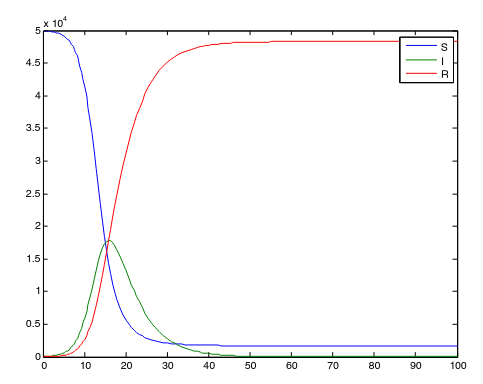
\includegraphics[width=\columnwidth]{Modelo SIR.png}
    \caption{Grafica de un Modelo SIR de un problema concreto \cite{weiss_2013}}
    \label{grafico modelo sir}
\end{figure}

En la figura \ref{grafico modelo sir} podemos apreciar una simulación calculada para un modelo matemático SIR determinado. Dentro de esta, podemos apreciar las tres ecuaciones que componen al modelo, y como estas cambiar a lo largo del tiempo.

\subsection{Modelo Matemático de SEIR}
\subsection{Modelo de Carga Potencial Máxima}

\subsection{Modelo de Gompertz}
El modelo de Gompertz, también llamado curva de Gompertz o función de Gompertz, es un modelo matemático para una serie temporal. La función es de tipo sigmoidea, y describe un crecimiento lengo en un periodo inicial y final, con uno más explosivo en un punto medio de la misma.

Inicialmente fue creada por Benjamin Gompertz para detallar su ley de la mortalidad humana, que se basa en un supuesto de que la resistencia de una persona a la muerte disminuye a medida que aumentan sus años, y fue descrito de la siguiente manera:

\begin{equation}
    N(t) = N(0) exp( -c ( exp(at) - 1))
\end{equation}

En esta ecuación, $N(t)$ representa un numero de individuos en un tiempo determinado $t$, por lo mismo, $N(0)$ representa la población inicial. $a$ denota una asíntota, $b$ y $c$ son valores positivos, que representan el desplazamiento a través del eje de las abcisas y la tasa de crecimiento, respectivamente. $exp$ denota la función exponencial.

\begin{figure*}
    \includegraphics[width=\textwidth]{casos diarios españa.png}
    \caption{Casos diarios de españa entre Marzo y Julio de 2020, fuente: cnecovid.isciii.es}
    \label{diarios españa}
\end{figure*}

En la publicación hecha por Sánchez-Villegas y colaboradores\cite{sanchez-villegas_codina_2020}, creada durante el año 2020, ellos decidieron utilizar el modelo de Gompertz para hacer una predicción del comportamiento de la epidemia de COVID-19 en España. Utilizando los datos de casos confirmados durante 47 días, generaron una curva de Gompertz que se ajustara lo más posible a sus datos.

¿Fue realmente acertado? Si bien, con la perspectiva inicial de dos años a futuro con respecto de esta publicación no lo parece para nada, contextualizando un poco a los datos que se tenían en ese momento podemos notar que la predicción fue, de hecho, relativamente acertada. En la figura \ref{diarios españa} podemos observar los casos diarios que se observan a lo largo del país entre las fechas de Marzo de 2020 hasta Julio del mismo año. La predicción inicial hecha por Sánchez-Villegas y colaboradores solo contemplaba datos hasta el 30 de abril de ese año, y contaba con solo 47 días de información, sin embargo, lograron demostrar que el pico de infección de españa llegó, efectivamente, en marzo de ese año, y que los contagios diarios iban extinguiendose.

Por desgracia, esta predicción cayó a mitades de Julio de 2020 y otras veces a futuro con la aparición de nuevas variantes y nuevos picos de infección en España y otros países del mundo. Aún así, el uso de este modelo predictivo en España y, según el autor, en la provincia de Hubei, donde ocurrió el primer caso de COVID, probó ser acertado para el corto plazo (Escala de Meses).

\subsection{Modelo de Holt}
\begin{figure*}
    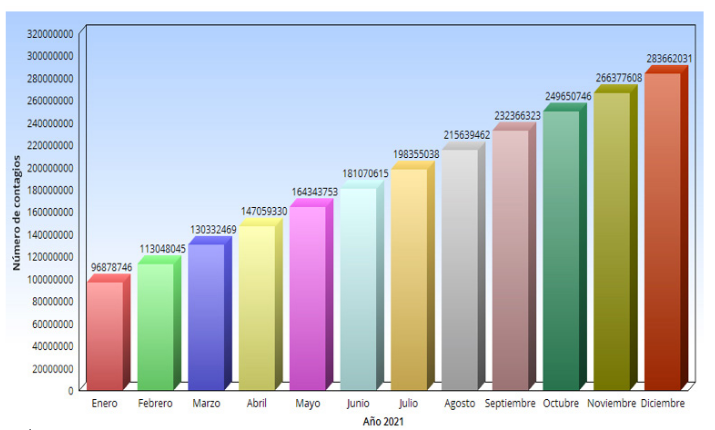
\includegraphics[width=\textwidth]{holtz.png}
    \caption{Predicción de número de contagios a nivel mundial utilizando el modelo de Holtz. Fuente: \cite{diazpinzon_2020}}
    \label{holtz}
\end{figure*}

El modelo de Holt, similar al modelo de Gompertz, es un modelo conocido por ser una modificación al modelo de suavización exponencial simple, a través de una constante de suavización $\delta$. Este modelo es expresado matemáticamente por la siguiente expresión:

\begin{equation*}
    Y_t = L_t + p T_t
\end{equation*}

Donde:
\begin{itemize}
    \item $Y_t$: valor pronosticado para el periodo $t$.
    \item $L$: valor estimado para el periodo $t$.
    \item $T_t$: valor de la tendencia para el periodo $t$.
    \item $p$: valor a pronosticar en el futuro.
\end{itemize}

Esta variable $L$ es definible bajo la siguiente equación:

\begin{equation*}
    L_t = \alpha Y_{t-1} + (1-\alpha)(L_{t-1} + T_{t-1})
\end{equation*}

Donde:
\begin{itemize}
    \item $\alpha$: constante de suavización, cuyo valor se encuentra entre 0 y 1.
    \item $Y_{t-1}$: valor de la variable pronostricada en el periodo anterior.
\end{itemize}

A su vez, la variable $T$ es definida de la siguiente manera:
\begin{equation*}
    T_t = \beta (L_t - L_{t-1}) + T_{t-1} (1 - \beta)
\end{equation*}

Donde:
\begin{itemize}
    \item $\beta$: es una constante de suavización por modificación de la tendencia, también restringido entre 0 y 1.
\end{itemize}

Este modelo fue utilizado por el autor Díaz Pinzón, J. E., en su documento "Predicción del COVID-19 a nivel mundial para el año 2021"\cite{diazpinzon_2020}. La predicción resultante puede ser encontrada en la figura \ref{holtz}

\section{Resultados de las simulaciones}



% Esta debería ser la última sección, donde se incluye el
% la conclusión a la que se llegó con el trabajo.

\section{conclusión}
En este trabajo aprendí muchito y lo pasé muy bien


% ------------------------------------------------------------------------------
%
%   La siguiente sección contiene el resto de la plantilla para el estandar IEEE
%
% -------------------------------------------------------------------------------


% \section{Ease of Use}

% \subsection{Maintaining the Integrity of the Specifications}

% The IEEEtran class file is used to format your paper and style the text. All margins, 
% column widths, line spaces, and text fonts are prescribed; please do not 
% alter them. You may note peculiarities. For example, the head margin
% measures proportionately more than is customary. This measurement 
% and others are deliberate, using specifications that anticipate your paper 
% as one part of the entire proceedings, and not as an independent document. 
% Please do not revise any of the current designations.

% \section{Prepare Your Paper Before Styling}
% Before you begin to format your paper, first write and save the content as a 
% separate text file. Complete all content and organizational editing before 
% formatting. Please note sections \ref{AA}--\ref{SCM} below for more information on 
% proofreading, spelling and grammar.

% Keep your text and graphic files separate until after the text has been 
% formatted and styled. Do not number text heads---{\LaTeX} will do that 
% for you.

% \subsection{Abbreviations and Acronyms}\label{AA}
% Define abbreviations and acronyms the first time they are used in the text, 
% even after they have been defined in the abstract. Abbreviations such as 
% IEEE, SI, MKS, CGS, ac, dc, and rms do not have to be defined. Do not use 
% abbreviations in the title or heads unless they are unavoidable.

% \subsection{Units}
% \begin{itemize}
% \item Use either SI (MKS) or CGS as primary units. (SI units are encouraged.) English units may be used as secondary units (in parentheses). An exception would be the use of English units as identifiers in trade, such as ``3.5-inch disk drive''.
% \item Avoid combining SI and CGS units, such as current in amperes and magnetic field in oersteds. This often leads to confusion because equations do not balance dimensionally. If you must use mixed units, clearly state the units for each quantity that you use in an equation.
% \item Do not mix complete spellings and abbreviations of units: ``Wb/m\textsuperscript{2}'' or ``webers per square meter'', not ``webers/m\textsuperscript{2}''. Spell out units when they appear in text: ``. . . a few henries'', not ``. . . a few H''.
% \item Use a zero before decimal points: ``0.25'', not ``.25''. Use ``cm\textsuperscript{3}'', not ``cc''.)
% \end{itemize}

% \subsection{Equations}
% Number equations consecutively. To make your 
% equations more compact, you may use the solidus (~/~), the exp function, or 
% appropriate exponents. Italicize Roman symbols for quantities and variables, 
% but not Greek symbols. Use a long dash rather than a hyphen for a minus 
% sign. Punctuate equations with commas or periods when they are part of a 
% sentence, as in:
% \begin{equation}
% a+b=\gamma\label{eq}
% \end{equation}

% Be sure that the 
% symbols in your equation have been defined before or immediately following 
% the equation. Use ``\eqref{eq}'', not ``Eq.~\eqref{eq}'' or ``equation \eqref{eq}'', except at 
% the beginning of a sentence: ``Equation \eqref{eq} is . . .''

% \subsection{\LaTeX-Specific Advice}

% Please use ``soft'' (e.g., \verb|\eqref{Eq}|) cross references instead
% of ``hard'' references (e.g., \verb|(1)|). That will make it possible
% to combine sections, add equations, or change the order of figures or
% citations without having to go through the file line by line.

% Please don't use the \verb|{eqnarray}| equation environment. Use
% \verb|{align}| or \verb|{IEEEeqnarray}| instead. The \verb|{eqnarray}|
% environment leaves unsightly spaces around relation symbols.

% Please note that the \verb|{subequations}| environment in {\LaTeX}
% will increment the main equation counter even when there are no
% equation numbers displayed. If you forget that, you might write an
% article in which the equation numbers skip from (17) to (20), causing
% the copy editors to wonder if you've discovered a new method of
% counting.

% {\BibTeX} does not work by magic. It doesn't get the bibliographic
% data from thin air but from .bib files. If you use {\BibTeX} to produce a
% bibliography you must send the .bib files. 

% {\LaTeX} can't read your mind. If you assign the same label to a
% subsubsection and a table, you might find that Table I has been cross
% referenced as Table IV-B3. 

% {\LaTeX} does not have precognitive abilities. If you put a
% \verb|\label| command before the command that updates the counter it's
% supposed to be using, the label will pick up the last counter to be
% cross referenced instead. In particular, a \verb|\label| command
% should not go before the caption of a figure or a table.

% Do not use \verb|\nonumber| inside the \verb|{array}| environment. It
% will not stop equation numbers inside \verb|{array}| (there won't be
% any anyway) and it might stop a wanted equation number in the
% surrounding equation.

% \subsection{Some Common Mistakes}\label{SCM}
% \begin{itemize}
% \item The word ``data'' is plural, not singular.
% \item The subscript for the permeability of vacuum $\mu_{0}$, and other common scientific constants, is zero with subscript formatting, not a lowercase letter ``o''.
% \item In American English, commas, semicolons, periods, question and exclamation marks are located within quotation marks only when a complete thought or name is cited, such as a title or full quotation. When quotation marks are used, instead of a bold or italic typeface, to highlight a word or phrase, punctuation should appear outside of the quotation marks. A parenthetical phrase or statement at the end of a sentence is punctuated outside of the closing parenthesis (like this). (A parenthetical sentence is punctuated within the parentheses.)
% \item A graph within a graph is an ``inset'', not an ``insert''. The word alternatively is preferred to the word ``alternately'' (unless you really mean something that alternates).
% \item Do not use the word ``essentially'' to mean ``approximately'' or ``effectively''.
% \item In your paper title, if the words ``that uses'' can accurately replace the word ``using'', capitalize the ``u''; if not, keep using lower-cased.
% \item Be aware of the different meanings of the homophones ``affect'' and ``effect'', ``complement'' and ``compliment'', ``discreet'' and ``discrete'', ``principal'' and ``principle''.
% \item Do not confuse ``imply'' and ``infer''.
% \item The prefix ``non'' is not a word; it should be joined to the word it modifies, usually without a hyphen.
% \item There is no period after the ``et'' in the Latin abbreviation ``et al.''.
% \item The abbreviation ``i.e.'' means ``that is'', and the abbreviation ``e.g.'' means ``for example''.
% \end{itemize}
% An excellent style manual for science writers is \cite{b7}.

% \subsection{Authors and Affiliations}
% \textbf{The class file is designed for, but not limited to, six authors.} A 
% minimum of one author is required for all conference articles. Author names 
% should be listed starting from left to right and then moving down to the 
% next line. This is the author sequence that will be used in future citations 
% and by indexing services. Names should not be listed in columns nor group by 
% affiliation. Please keep your affiliations as succinct as possible (for 
% example, do not differentiate among departments of the same organization).

% \subsection{Identify the Headings}
% Headings, or heads, are organizational devices that guide the reader through 
% your paper. There are two types: component heads and text heads.

% Component heads identify the different components of your paper and are not 
% topically subordinate to each other. Examples include Acknowledgments and 
% References and, for these, the correct style to use is ``Heading 5''. Use 
% ``figure caption'' for your Figure captions, and ``table head'' for your 
% table title. Run-in heads, such as ``Abstract'', will require you to apply a 
% style (in this case, italic) in addition to the style provided by the drop 
% down menu to differentiate the head from the text.

% Text heads organize the topics on a relational, hierarchical basis. For 
% example, the paper title is the primary text head because all subsequent 
% material relates and elaborates on this one topic. If there are two or more 
% sub-topics, the next level head (uppercase Roman numerals) should be used 
% and, conversely, if there are not at least two sub-topics, then no subheads 
% should be introduced.

% \subsection{Figures and Tables}
% \paragraph{Positioning Figures and Tables} Place figures and tables at the top and 
% bottom of columns. Avoid placing them in the middle of columns. Large 
% figures and tables may span across both columns. Figure captions should be 
% below the figures; table heads should appear above the tables. Insert 
% figures and tables after they are cited in the text. Use the abbreviation 
% ``Fig.~\ref{fig}'', even at the beginning of a sentence.

% \begin{table}[htbp]
% \caption{Table Type Styles}
% \begin{center}
% \begin{tabular}{|c|c|c|c|}
% \hline
% \textbf{Table}&\multicolumn{3}{|c|}{\textbf{Table Column Head}} \\
% \cline{2-4} 
% \textbf{Head} & \textbf{\textit{Table column subhead}}& \textbf{\textit{Subhead}}& \textbf{\textit{Subhead}} \\
% \hline
% copy& More table copy$^{\mathrm{a}}$& &  \\
% \hline
% \multicolumn{4}{l}{$^{\mathrm{a}}$Sample of a Table footnote.}
% \end{tabular}
% \label{tab1}
% \end{center}
% \end{table}

% \begin{figure}[htbp]
% \caption{Example of a figure caption.}
% \label{fig}
% \end{figure}

% Figure Labels: Use 8 point Times New Roman for Figure labels. Use words 
% rather than symbols or abbreviations when writing Figure axis labels to 
% avoid confusing the reader. As an example, write the quantity 
% ``Magnetization'', or ``Magnetization, M'', not just ``M''. If including 
% units in the label, present them within parentheses. Do not label axes only 
% with units. In the example, write ``Magnetization (A/m)'' or ``Magnetization 
% \{A[m(1)]\}'', not just ``A/m''. Do not label axes with a ratio of 
% quantities and units. For example, write ``Temperature (K)'', not 
% ``Temperature/K''.

% \section*{Acknowledgment}

% The preferred spelling of the word ``acknowledgment'' in America is without 
% an ``e'' after the ``g''. Avoid the stilted expression ``one of us (R. B. 
% G.) thanks $\ldots$''. Instead, try ``R. B. G. thanks$\ldots$''. Put sponsor 
% acknowledgments in the unnumbered footnote on the first page.


% Please number citations consecutively within brackets \cite{b1}. The 
% sentence punctuation follows the bracket \cite{b2}. Refer simply to the reference 
% number, as in \cite{b3}---do not use ``Ref. \cite{b3}'' or ``reference \cite{b3}'' except at 
% the beginning of a sentence: ``Reference \cite{b3} was the first $\ldots$''

% Number footnotes separately in superscripts. Place the actual footnote at 
% the bottom of the column in which it was cited. Do not put footnotes in the 
% abstract or reference list. Use letters for table footnotes.

% Unless there are six authors or more give all authors' names; do not use 
% ``et al.''. Papers that have not been published, even if they have been 
% submitted for publication, should be cited as ``unpublished'' \cite{b4}. Papers 
% that have been accepted for publication should be cited as ``in press'' \cite{b5}. 
% Capitalize only the first word in a paper title, except for proper nouns and 
% element symbols.

% For papers published in translation journals, please give the English 
% citation first, followed by the original foreign-language citation \cite{b6}.

% \pagebreak
\bibliographystyle{plain}
\bibliography{bibliografia}

\end{document}
